\documentclass[11pt,a4paper]{article}

% ─── Packages ───
\usepackage[utf8]{inputenc}
\usepackage[T1]{fontenc}
\usepackage{lmodern}
\usepackage[margin=1in]{geometry}
\usepackage{amsmath,amssymb,amsthm}
\usepackage{graphicx}
\usepackage{booktabs}
\usepackage{hyperref}
\usepackage{cleveref}
\usepackage{enumitem}
\usepackage{xcolor}
\usepackage{microtype}
\usepackage{natbib}
% \usepackage{svg}  % for direct SVG inclusion (requires --shell-escape)
% Using \includegraphics with PDF figures for arXiv compatibility
\usepackage{float}
\usepackage{caption}
\usepackage{subcaption}
\usepackage{array}
\usepackage{multirow}
\usepackage{tabularx}

% ─── Theorem-like environments ───
\newtheorem{theorem}{Theorem}
\newtheorem{definition}{Definition}
\newtheorem{corollary}{Corollary}

% ─── Custom commands ───
\newcommand{\ket}[1]{|#1\rangle}
\newcommand{\chat}{\hat{C}}
\newcommand{\CAS}{\mathrm{CAS}}
\newcommand{\CD}{\mathrm{CD}}

% ─── Metadata ───
\title{Structural Properties of LLM Semantic Processing:\\ Measurement, Prediction, and Inexpressibility}
\author{Trian \and Claude (Anthropic)}
\date{}

\begin{document}
\maketitle

% ═══════════════════════════════════════════════════════
% ABSTRACT
% ═══════════════════════════════════════════════════════
\begin{abstract}
Large Language Models are typically used as text generators steered by prompts. We propose they also exhibit measurable \emph{structural properties}---superposition of meanings, interference between contexts, and phase transitions at critical thresholds---that can be formalized and exploited. Through 25 controlled experiments ($\sim$7,500 API calls across Claude, GPT-4o-mini, and Gemini-2.5-flash), we establish three results. \textbf{First}, LLMs exhibit semantic superposition, interference, and phase transitions that are universal across architectures, predictable via a Phase Transition Condition ($\CAS < 0.4 \wedge \CD > 0.5$, validated on initial test set; structural form preserved cross-model though thresholds are model-dependent), and composable into five primitive operations (\textsc{Superpose}, \textsc{Interfere}, \textsc{Reframe}, \textsc{Synthesize}, \textsc{Validate}). \textbf{Second}, these operations solve ``dissolution problems''---finding hidden assumptions in apparent binary dilemmas---that formal programs (operating on syntactic content without learned semantic representations) structurally cannot express: programming-like constraints yield 0\% dissolution while semantic computation yields 70--100\%, confirmed across three model families and generalized across six non-ethical domains with full cross-model replication on all 7 problems (Claude 81\%, GPT 63\%, Gemini 56\% via composition vs 0\% constrained---universally, $N=1{,}050$ total runs). We provide a formal inexpressibility argument (conditional on the empirically supported premise that hidden assumptions are not syntactically derivable) connecting dissolution to the frame problem. \textbf{Third}, dissolution is selective (genuine on false binaries, artificial on true binaries, gap $= 1.625$), and self-detection requires adversarial evaluation stance---neutral and self-assessment stances are uniformly overconfident. These findings identify a class of problems---where the output space is undefined before computation---for which LLM structural properties provide capabilities that formal computation lacks.
\end{abstract}

% ═══════════════════════════════════════════════════════
\section{Introduction}
% ═══════════════════════════════════════════════════════

\subsection{Motivation}

Large Language Models are typically viewed through two lenses: as statistical text predictors, or as tools to be steered via prompt engineering. Both views treat the model as a black box whose internal properties are incidental to its use.

We propose a third view: LLMs possess \textbf{structural computational properties}---superposition of meanings, interference between contexts, phase transitions at critical thresholds, and emergent outputs from composed operations---that are not artifacts but exploitable features. We formalize these properties as measurable operations and demonstrate they enable solving a specific class of problems (dissolution of false binaries) that formal programs structurally cannot express.

We use the term \textbf{Semantic Computing} to refer to computation that exploits these structural properties. Whether this constitutes a full ``computing paradigm'' comparable to classical or quantum computing remains an open question requiring substantially more theoretical development. What we establish empirically is that these properties exist, are measurable, are predictable, and enable a specific form of computation that formal programs cannot replicate.

\subsection{Claims and Scope}

This paper makes the following empirical claims, each backed by controlled experiments:

\begin{enumerate}[leftmargin=*]
\item \textbf{Semantic Superposition is real and measurable.} A token in isolation exists in a probability distribution over multiple meanings, with attractor biases (Experiment~A).

\item \textbf{Context operators reshape distributions continuously}, not discretely. This ``contextual collapse'' is reversible, unlike quantum measurement (Experiments~A, B).

\item \textbf{Semantic interference is non-linear.} Combined contexts produce emergent output components that exist in neither individual context (Experiments~B, D, E, F, G).

\item \textbf{Phase transitions occur at critical context ratios}, with abrupt shifts in output character. These transitions are universal across model architectures (Experiments~E, H) but depend on concept-context geometry, not fixed constants (Experiment~I).

\item \textbf{Concept Attractor Strength (CAS)} quantifies a concept's resistance to contextual reshaping and, combined with Context Distance (CD), predicts whether phase transitions will occur (Experiment~J). Cross-model validation (Experiment~J2 on GPT-4o-mini, Experiment~R on Gemini-2.5-flash) reveals a three-way CAS gradient: GPT (most rigid) $>$ Claude (intermediate) $>$ Gemini (most flexible). Lower CAS correlates with meta-constructive interference, establishing CAS as a predictive metric for model type.

\item \textbf{Meta-constructive interference}---where opposing contexts elevate output to higher abstraction---exists on a spectrum. Claude exhibits it strongly, Gemini moderately, and GPT-4o-mini not at all (Experiments~H, R).

\item \textbf{Semantic gates compose into circuits} with measurable cross-domain inheritance and cumulative emergence (Experiments~D, G).

\item \textbf{Semantic circuits produce measurably better output} than single prompts on decision problems with moral tension---and this advantage comes from the opposing-context \emph{structure}, not from additional computation (Experiments~K, K2).

\item \textbf{Meta-constructive interference is a synthesis-stage property.} Cross-model circuits reveal that the model performing synthesis determines output quality---not the models generating perspectives. Type-D perspectives fed to a Type-M synthesizer produce meta-constructive output; Type-M perspectives fed to a Type-D synthesizer do not (Experiment~L).

\item \textbf{Semantic operations are LLM properties, not circuit properties.} Single prompts can achieve superposition and emergence comparable to circuits (Experiments~M, M2). Circuits are measurement apparatus and reliability organizers---not the source of the computational advantage.

\item \textbf{Semantic computation solves problems programming structurally cannot express.} On ``dissolution problems''---finding hidden assumptions in binary dilemmas---programming-like methods (forced-choice, weighted-analysis) achieve 0\% dissolution, while semantic methods achieve 70--100\% (Experiment~N, Claude; Experiment~S, Gemini). This pattern is universal across model families and generalizes across six non-ethical domains with cross-model replication: Claude 81\%, GPT-4o-mini 64\%, Gemini 50\% via composition vs 0\% constrained universally (Experiment~U), demonstrating inexpressibility: certain problems require meaning navigation that formal computation cannot represent.

\item \textbf{Dissolution is a universal LLM capability.} GPT-4o-mini (Type-D) achieves 3/3 dissolution when the first four primitives are organized. Gemini-2.5-flash (Type-M moderate) achieves 100\% dissolution via semantic circuit and 70\% via free-response, with 0\% under constrained methods (Experiment~S)---confirming dissolution is not model-specific. Dissolution \emph{shape} differs by model type: Type-M produces meta-insight, Type-D produces actionable resolution (\S\ref{sec:cross-model-dissolution}).

\item \textbf{Dissolution has empirical boundary conditions.} On true binary problems (physical scarcity, mechanism constraints), dissolution is attempted but artificial (\textsc{Genuine} $= 1.75/5$). On false binary problems, dissolution is genuine (\textsc{Genuine} $= 3.375/5$). The gap ($1.625$) demonstrates dissolution is \emph{selective}---it works where hidden assumptions exist and fails where the binary is real. Critically, the circuit does not self-detect failure, requiring an external validation metric (\S\ref{sec:boundary}).

\item \textbf{Self-detection requires separation of production and evaluation.} A fifth primitive, \textsc{Validate}, placed after \textsc{Synthesize}, is the only mechanism that successfully detects artificial dissolution (self-\textsc{Genuine} $= 1.5$ on true binaries). Inline self-assessment during synthesis fails completely (self $= 4.0$ regardless of problem type). Pre-classification achieves 100\% accuracy in identifying true binaries but does not prevent artificial dissolution (\S\ref{sec:validate}).

\item \textbf{Evaluation quality depends on stance, not separation.} Cross-domain testing (math, factual, logic) shows self-assessment and neutral evaluation both produce self $= 5$ when wrong (100\% overconfidence). Only adversarial evaluation catches errors (self $= 2$ when wrong). However, adversarial stance rejects 58\% of correct answers. \textsc{Validate} works on dissolution because high error rate makes the adversarial trade-off favorable (\S\ref{sec:eval-stance}).
\end{enumerate}

\subsection{Scope and Clarifications}

\begin{itemize}[leftmargin=*]
\item \textbf{Relationship to prompt engineering.} Our five primitives are implemented as structured prompts---this is an implementation reality, not a weakness. The contribution is not a new prompting technique but the identification of measurable structural properties (CAS, phase transitions, boundary selectivity) and a problem class (dissolution) that these properties enable. Experiment~K2 shows that multi-step prompting \emph{without} opposing contexts performs no better than a single prompt, suggesting the structure matters more than the prompting.

\item \textbf{Relationship to quantum computing.} We use physics-inspired terminology (superposition, interference, phase transitions) because the structural parallels are informative, but the analogy has strict limits. Many properties differ fundamentally (\S\ref{sec:quantum-diff}: reversible collapse, continuous superposition, no no-cloning constraint). We do not claim LLMs are quantum systems or that semantic computing is quantum computing. The analogy is a scaffolding for intuition, not a theoretical claim.

\item \textbf{Empirical grounding.} Every claim is backed by controlled experiments with specific measurements. Where evidence is limited, we note this explicitly.
\end{itemize}

% ═══════════════════════════════════════════════════════
\section{Related Work}
% ═══════════════════════════════════════════════════════

\textbf{Prompt engineering and chain-of-thought.} The discovery that LLMs can be steered via natural language instructions \citep{brown2020language} and that chain-of-thought prompting improves reasoning \citep{wei2022chain} established that context structure affects output quality. Follow-up work on tree-of-thought \citep{yao2023tree}, self-consistency \citep{wang2023self}, and multi-agent debate \citep{du2023improving,liang2023encouraging} shows that \emph{organizing} LLM computation matters. Our work extends this: we formalize context effects as measurable operators with phase transitions and composability, and identify a class of problems (dissolution) where structured semantic operations succeed but programming-like constraints fail entirely (0\% vs 100\%).

\textbf{LLM self-evaluation and calibration.} Work on LLM self-assessment shows models are often poorly calibrated \citep{kadavath2022language,lin2022teaching}. Reflexion \citep{shinn2023reflexion} and self-refine \citep{madaan2023self} show iterative self-evaluation can improve outputs. Our Experiments~P, Q, and Q2 contribute a specific finding: evaluation quality depends on \emph{stance} (adversarial vs neutral), not on separation of generation from evaluation. Neutral self-assessment is uniformly overconfident; only adversarial evaluation catches errors---at the cost of high false negatives (58\%).

\textbf{Mechanistic interpretability.} Recent work on transformer internals---superposition in neural networks \citep{elhage2022toy}, sparse autoencoders \citep{cunningham2023sparse}, circuit-level analysis \citep{conmy2023towards}---examines \emph{how} models compute. Our work is complementary: we characterize \emph{what} the computation produces at the behavioral level, seeking exploitable structural properties rather than mechanistic explanations. The relationship is analogous to thermodynamics (behavioral laws) vs statistical mechanics (microscopic explanations).

\textbf{Analogies to physics.} Drawing parallels between neural networks and physical systems is established---statistical mechanics of learning \citep{bahri2020statistical}, phase transitions in training dynamics \citep{power2022grokking}, and neural scaling laws \citep{kaplan2020scaling}. Our contribution is specific: we identify \emph{behavioral} properties (superposition, interference, phase transitions) at the \emph{output} level that can be composed into a computing paradigm, and demonstrate these enable solving problems that formal computation cannot express.

\textbf{Quantum-inspired NLP.} Quantum-inspired approaches to information retrieval and NLP \citep{vanrijsbergen2004geometry,melucci2015introduction} use quantum formalism to model semantic spaces. Our work differs fundamentally: we do not impose quantum formalism on language---we observe LLM behavior, find structural similarities, and formalize them independently, noting critical differences (\S\ref{sec:quantum-diff}: reversible collapse, continuous superposition, meta-constructive interference, no no-cloning constraint).

\textbf{Frame problem and knowledge representation.} The frame problem \citep{mccarthy1969some}---the difficulty of representing what does NOT change or is NOT stated in formal systems---is a foundational challenge in AI. Our inexpressibility proof (\S\ref{sec:inexpressibility}) connects dissolution to the frame problem: hidden assumptions are precisely what is not stated in the input, making dissolution a specific instance of the frame problem applied to meaning navigation.

\textbf{Lateral thinking and creativity.} De Bono's concept of ``lateral thinking'' \citep{debono1967lateral}---restructuring problems rather than solving them within their given frame---is the closest conceptual precursor to dissolution. Our contribution is to formalize this as a \emph{computational} operation with measurable properties (\textsc{Genuine} score, boundary conditions), identify primitive operations that produce it (5 primitives), and demonstrate it is structurally inexpressible in formal programs.

\textbf{Relationship to prompt engineering.} We acknowledge that our five primitives are implemented as structured prompts. The line between ``semantic computing'' and ``sophisticated prompt engineering'' is a legitimate concern. We argue the distinction lies not in the implementation mechanism but in what is measured and predicted: CAS quantifies a concept's resistance to contextual reshaping \emph{before} any prompt is designed; the Phase Transition Condition predicts qualitative output changes from input parameters alone; boundary selectivity (\textsc{Genuine} gap $= 1.625$) demonstrates the operations discriminate between problem types. These are structural properties of the LLM, revealed through prompting but not reducible to prompting technique. A useful analogy: thermodynamics describes structural properties of physical systems measured through experiments---the experiments are not the properties.

% ═══════════════════════════════════════════════════════
\section{Theoretical Framework \& Experimental Evidence}
% ═══════════════════════════════════════════════════════

\subsection{Semantic Space}

We define Semantic Space $\mathbf{S}$ as the high-dimensional vector space ($d = 4096, 8192+$) in which each point represents a semantic state. In transformer architectures, this corresponds to the embedding/hidden state space.

We borrow Dirac notation for structural correspondence: $\ket{s} \in \mathbf{S}$ denotes a semantic state.

\subsection{Semantic Superposition}

When a model receives an ambiguous input without context, the output probability distribution spans multiple meanings simultaneously.

\begin{definition}
A semantic state $\ket{s}$ is in superposition when it can be expressed as a weighted distribution over meaning attractors:
\begin{equation}
\ket{s} = \sum_i \alpha_i \ket{m_i}, \quad \text{where } \sum_i |\alpha_i|^2 = 1
\end{equation}
\end{definition}

Unlike quantum superposition, semantic superposition is:
\begin{itemize}
\item \textbf{Not equiprobable}---some meanings have stronger attractors (e.g., ``bank'' $\to$ financial meaning 93\% of the time)
\item \textbf{Continuous}---thousands of meaning dimensions, not binary
\item \textbf{Observable without destruction}---sampling does not collapse the underlying distribution
\end{itemize}

\textbf{Evidence (Experiment~A):} Testing ambiguous tokens (``crane'', ``bank'', ``light'') across 100+ samples:
\begin{itemize}
\item ``crane'' $\to$ ``lifted'' 63\%, remaining distributed across bird/machine meanings
\item ``bank'' $\to$ ``deposit'' 93\% (very strong attractor)
\item ``light'' $\to$ broad distribution, entropy 0.76 (weak attractors)
\end{itemize}

\subsection{Contextual Collapse}

A context operator $\chat$ reshapes the probability distribution over meanings:
\begin{equation}
\chat\ket{s} \to \ket{s'}
\end{equation}

\textbf{Key differences from quantum measurement:}
\begin{itemize}
\item \textbf{Reversible:} Applying a different context can shift the distribution again
\item \textbf{Continuous:} Collapse strength varies with context intensity
\item \textbf{Non-destructive:} The model's capacity for other meanings persists
\end{itemize}

\textbf{Evidence (Experiments~A, B):} Context ``construction site'' shifts ``crane'' from 63\% mechanical to $>$95\%. Context ``wetlands'' shifts to $>$90\% bird. The same input produces radically different outputs based purely on context operators.

\subsection{Semantic Interference}

When two context operators act simultaneously, the output is NOT the weighted average of individual outputs:
\begin{equation}
I(C_1, C_2, \alpha)\ket{s} \neq \alpha \cdot \chat_1\ket{s} + (1-\alpha) \cdot \chat_2\ket{s}
\end{equation}

The combined output contains \textbf{emergent components}---words, concepts, and framings that appear in neither individual context.

\textbf{Evidence (Experiment~B):}
\begin{itemize}
\item Cosine similarity between poet-only and biologist-only outputs: 0.002 (completely different)
\item Similarity between combined output and simple average: 0.47 (combined $\neq$ average)
\item Emergent words in combined output: ``starlight'', ``dressed'', ``transcendence''---absent from both individual contexts
\end{itemize}

\subsection{Phase Transitions}

As the context mixing ratio $\alpha$ varies from pure $C_1$ ($\alpha=1.0$) to pure $C_2$ ($\alpha=0.0$), output character does not shift linearly. Instead, \textbf{abrupt transitions} occur at critical thresholds.

\textbf{Evidence (Experiment~E, 220 data points; Experiment~H, cross-model):}

Three distinct phases emerge:
\begin{itemize}
\item \textbf{Phase~I} ($\alpha > \sim 0.7$): $C_1$ dominates completely. $C_2$ markers invisible.
\item \textbf{Phase~II} ($\sim 0.3 < \alpha < \sim 0.7$): Interference zone. Emergence peaks. Unique vocabulary maximizes.
\item \textbf{Phase~III} ($\alpha < \sim 0.3$): $C_2$ dominates completely. $C_1$ markers invisible.
\end{itemize}

Cross-model validation (Experiment~H):

\begin{table}[H]
\centering
\caption{Phase transitions across models.}
\begin{tabular}{lcc}
\toprule
\textbf{Model} & \textbf{Transition 1 (80$\to$60\%)} & \textbf{Transition 2 (40$\to$20\%)} \\
\midrule
Claude Haiku & 100\% $\to$ 54.5\% (45.5\% drop) & 46.2\% $\to$ 0\% (46.2\% drop) \\
GPT-4o-mini  & 100\% $\to$ 44.4\% (55.6\% drop) & 33.3\% $\to$ 0\% (33.3\% drop) \\
\bottomrule
\end{tabular}
\label{tab:phase-transitions}
\end{table}

Both models show transitions at the same ratio ranges, confirming this is a \textbf{universal property} of semantic space, not a model-specific artifact (Figure~\ref{fig:phase-diagram}).

\begin{figure}[H]
\centering
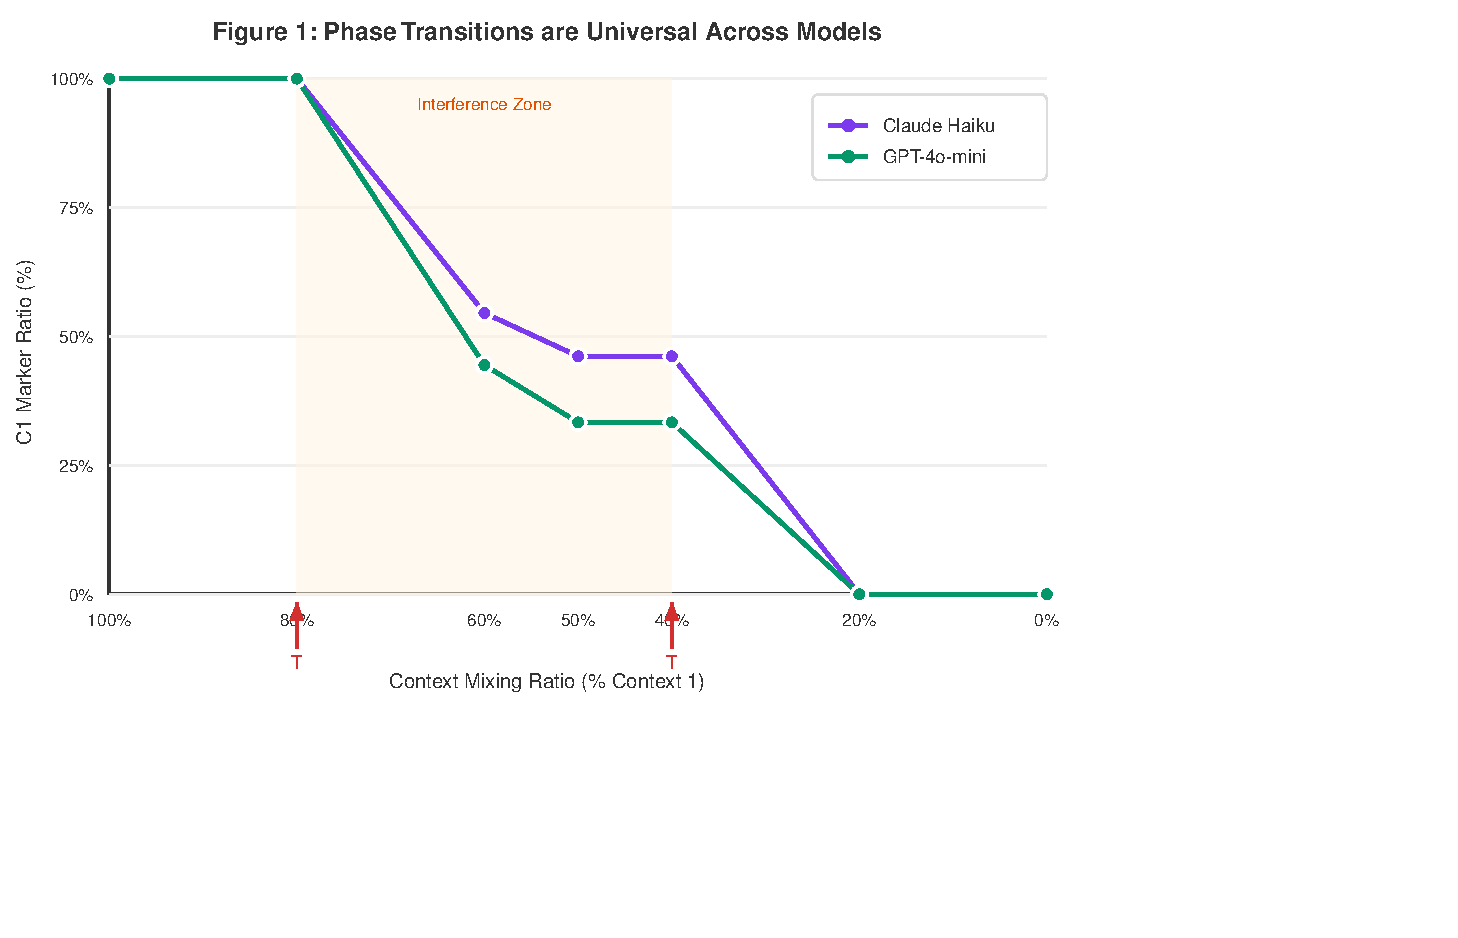
\includegraphics[width=\textwidth]{figures/fig1_phase_diagram.pdf}
\caption{Phase transitions are universal across models. Both Claude Haiku and GPT-4o-mini exhibit abrupt transitions at similar context mixing ratios.}
\label{fig:phase-diagram}
\end{figure}

\subsection{Concept Attractor Strength (CAS)}

Not all concepts respond equally to context operators. Some concepts have strong ``semantic mass''---they resist reshaping.

\begin{definition}
\begin{equation}
\CAS = 1 - \mathrm{AvgShift}, \quad \mathrm{AvgShift} = \mathrm{mean}\!\left(1 - \cos(\mathbf{f}_{\mathrm{baseline}}, \mathbf{f}_{\mathrm{context}_i})\right)
\end{equation}
where $\mathbf{f}_{\mathrm{baseline}}$ is the word frequency distribution with no context, and $\mathbf{f}_{\mathrm{context}_i}$ is the distribution under context~$i$. CAS measures how much context operators shift the output distribution from baseline---high CAS means the concept resists contextual reshaping.

\emph{Note:} Cross-model experiments (J2, R) use an entropy-weighted variant: $\CAS = \mathrm{ContextResistance} \times (1 - H_{\mathrm{norm}})$, where $H_{\mathrm{norm}}$ is the normalized Shannon entropy of the baseline distribution. This penalizes concepts with high baseline variability. The two formulations are equivalent when baseline entropy is low (most concepts); the entropy term provides additional discrimination for ambiguous concepts.
\end{definition}

\textbf{Evidence (Experiment~J, 8 concepts $\times$ 3 conditions $\times$ 15 samples = 360 calls):}

\begin{table}[H]
\centering
\caption{CAS measurements on Claude Haiku (Experiment~J). Thresholds: HIGH $> 0.5$, MEDIUM 0.25--0.5, LOW $< 0.25$.}
\begin{tabular}{lcll}
\toprule
\textbf{Concept} & \textbf{CAS} & \textbf{Level} & \textbf{Interpretation} \\
\midrule
money       & 0.879 & HIGH   & Almost impossible to reshape contextually \\
mathematics & 0.703 & HIGH   & Strong core identity across contexts \\
justice     & 0.638 & HIGH   & Moderate-high resistance \\
gravity     & 0.551 & HIGH   & Borderline---partially reshapeable \\
water       & 0.392 & MEDIUM & Context-sensitive \\
death       & 0.163 & LOW    & Highly reshapeable by context \\
love        & 0.147 & LOW    & Highly reshapeable by context \\
freedom     & 0.102 & LOW    & Most context-sensitive concept tested \\
\bottomrule
\end{tabular}
\label{tab:cas-claude}
\end{table}

\textbf{Cross-Model Validation (Experiment~J2, 20 concepts $\times$ 3 conditions $\times$ 15 samples = 900 calls, GPT-4o-mini):}

To test whether CAS generalizes across model architectures, we replicated and expanded the measurement from 8 to 20 concepts using GPT-4o-mini instead of Claude Haiku.

\begin{table}[H]
\centering
\caption{CAS cross-model comparison (Experiments~J, J2, R).}
\small
\begin{tabular}{lccccc}
\toprule
\textbf{Concept} & \textbf{CAS (Claude)} & \textbf{CAS (GPT)} & \textbf{CAS (Gemini)} & \textbf{CD (GPT)} & \textbf{Note} \\
\midrule
money       & 0.879 & 0.780 & 0.036 & 0.449 & Gemini extreme LOW \\
mathematics & 0.703 & 0.949 & 0.050 & 0.035 & Gemini extreme LOW \\
justice     & 0.638 & 0.805 & 0.001 & 0.067 & Gemini extreme LOW \\
gravity     & 0.551 & 0.628 & 0.069 & 0.426 & Gemini extreme LOW \\
water       & 0.392 & 0.411 & 0.020 & 0.883 & Gemini extreme LOW \\
death       & 0.163 & 0.447 & 0.027 & 0.951 & Three-way gradient \\
love        & 0.147 & 0.357 & 0.004 & 0.748 & Three-way gradient \\
freedom     & 0.102 & 0.658 & 0.003 & 0.889 & Three-way gradient \\
\midrule
\multicolumn{6}{l}{\emph{New concepts (GPT-4o-mini only, Gemini not tested):}} \\
hope        & ---   & 0.910 & ---   & 0.140 & HIGH, low CD \\
fear        & ---   & 0.899 & ---   & 0.105 & HIGH, low CD \\
family      & ---   & 0.846 & ---   & 0.311 & HIGH \\
power       & ---   & 0.839 & ---   & 0.125 & HIGH, low CD \\
home        & ---   & 0.823 & ---   & 0.219 & HIGH \\
war         & ---   & 0.595 & ---   & 0.619 & HIGH \\
beauty      & ---   & 0.574 & ---   & 0.617 & HIGH \\
light       & ---   & 0.499 & ---   & 1.000 & MEDIUM, extreme CD \\
fire        & ---   & 0.479 & ---   & 0.962 & MEDIUM, extreme CD \\
time        & ---   & 0.479 & ---   & 0.752 & MEDIUM \\
silence     & ---   & 0.475 & ---   & 1.000 & MEDIUM, extreme CD \\
truth       & ---   & 0.444 & ---   & 0.790 & MEDIUM \\
\bottomrule
\end{tabular}
\label{tab:cas-crossmodel}
\end{table}

\textbf{Key findings from J2 and R:}

\begin{enumerate}
\item \textbf{GPT-4o-mini is MORE context-resistant than Claude Haiku on most concepts.} This is the opposite of the naive expectation. Freedom: Claude 0.102 (LOW) vs GPT 0.658 (HIGH). Death: Claude 0.163 (LOW) vs GPT 0.447 (MEDIUM). On the 8 shared concepts, GPT has higher CAS in 6/8 cases (exceptions: money, water where values are similar).

\item \textbf{Gemini-2.5-flash is extremely context-sensitive---the lowest CAS across all three models.} All 8 concepts scored LOW (range: 0.001--0.069), with concepts like justice (0.001), freedom (0.003), and love (0.004) approaching zero. This reveals a \textbf{three-way CAS gradient}: GPT (most rigid) $>$ Claude (intermediate) $>$ Gemini (most flexible). The gradient is sharpest on abstract/emotional concepts: freedom shows GPT 0.658 $\to$ Claude 0.102 $\to$ Gemini 0.003, a 200x range. One contributing factor: Gemini-2.5-flash is a ``thinking'' model with extended internal reasoning, which may amplify context-sensitivity by reasoning more thoroughly about how each context reshapes the concept---effectively ``overthinking'' the adaptation. Additionally, the entropy-weighted CAS variant (used in J2/R) penalizes high baseline diversity, and Gemini's naturally verbose generation style may compound this effect.

\item \textbf{Claude is more ``semantically flexible'' on abstract/emotional concepts.} The largest CAS gaps occur for freedom (0.102 vs 0.658), death (0.163 vs 0.447), and love (0.147 vs 0.357)---all abstract or emotional concepts. Claude reshapes these concepts more readily under contextual pressure. Gemini extends this pattern further, suggesting context-sensitivity is a continuous model property, not binary.

\item \textbf{CD remains informative across models.} Context Distance identifies extreme divergence cases (silence: CD$=1.0$, light: CD$=1.0$, fire: CD$=0.962$) where contexts produce completely non-overlapping vocabulary, and alignment cases (power: CD$=0.125$, fear: CD$=0.105$, mathematics: CD$=0.035$) where both contexts generate similar responses.

\item \textbf{Phase Transition Condition applies differentially.} With the original thresholds ($\CAS < 0.4 \wedge \CD > 0.5$), Claude has 3 concepts in the transition zone (death, love, freedom), GPT has only 1 (love at CAS$=0.357$, CD$=0.748$), and Gemini has all 8 in the transition zone. This is consistent with each model's characteristic behavior.

\item \textbf{CAS differentiates models in a meaningful direction.} The three-way gradient (GPT $>$ Claude $>$ Gemini) correlates with meta-constructive behavior: both Claude (strong Type-M) and Gemini (moderate Type-M) have lower CAS than GPT (Type-D). Lower CAS---the willingness to \emph{reshape} concept representations under opposing contexts---appears to be a precondition for meta-constructive interference.
\end{enumerate}

See Figure~\ref{fig:cas-ranking} for a visual comparison.

\begin{figure}[H]
\centering
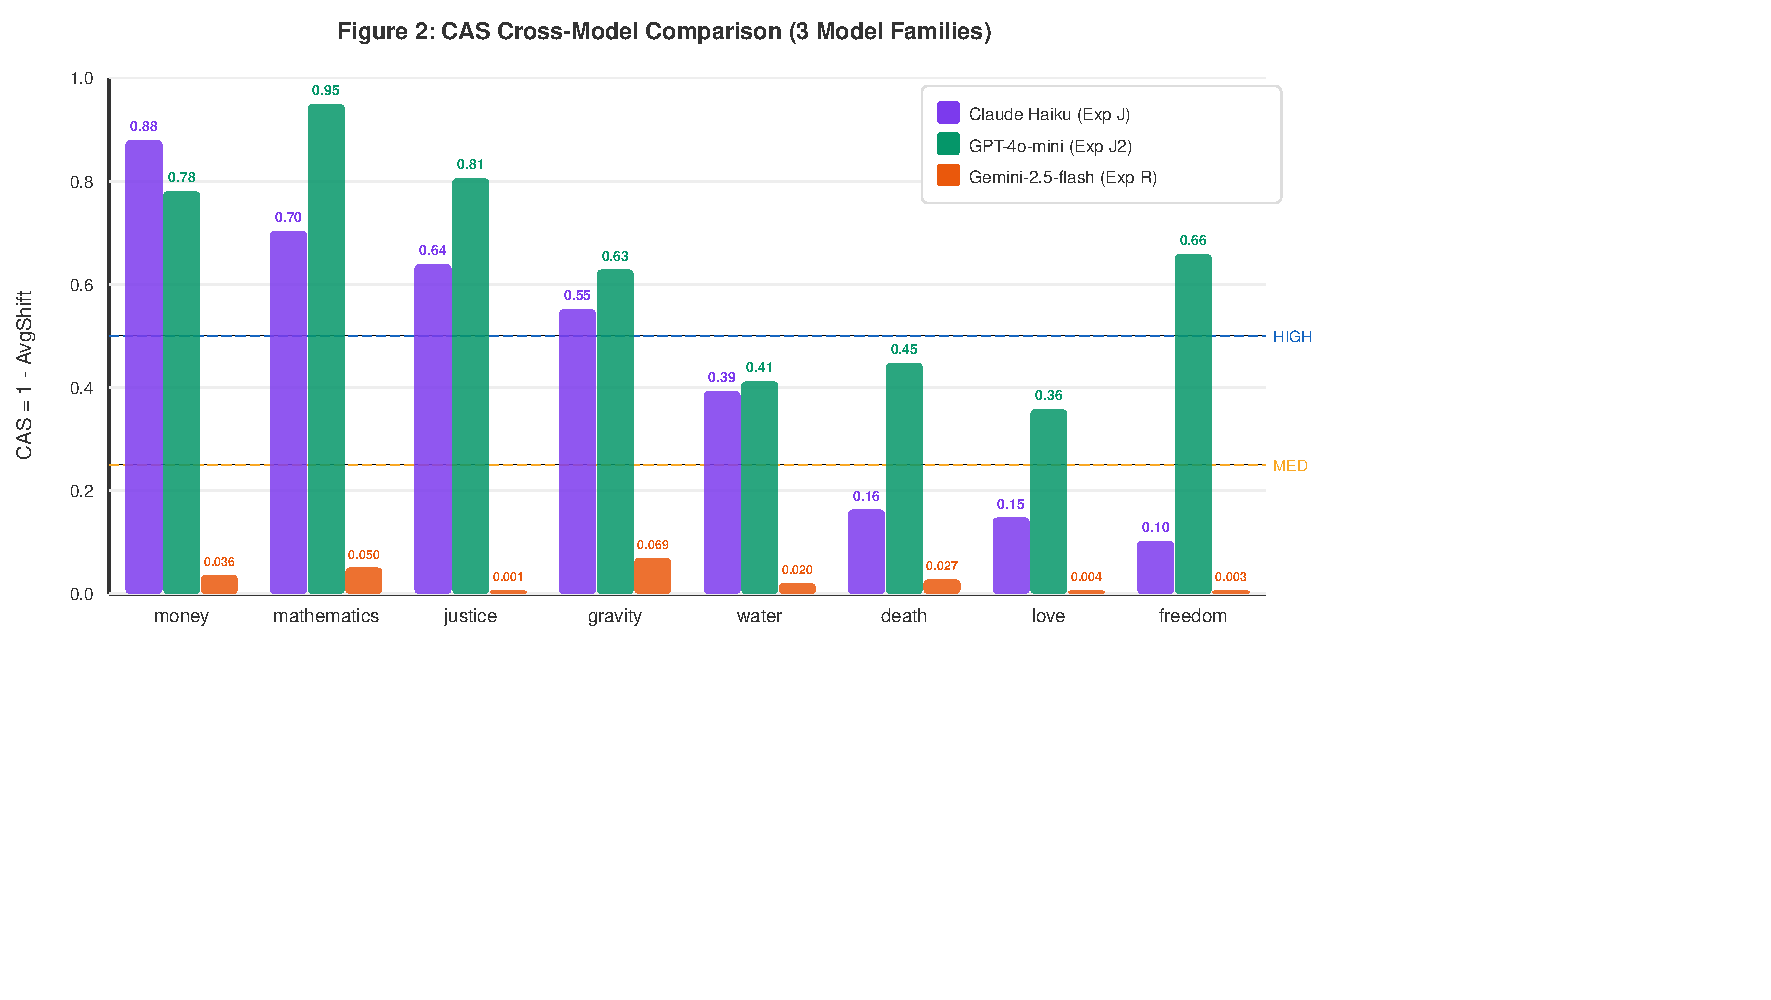
\includegraphics[width=\textwidth]{figures/fig2_cas_ranking.pdf}
\caption{CAS cross-model comparison across three model families. Claude Haiku (purple), GPT-4o-mini (green), Gemini-2.5-flash (orange). Gemini shows near-zero CAS on all concepts, revealing a three-way gradient: GPT (most rigid) $>$ Claude (intermediate) $>$ Gemini (most flexible).}
\label{fig:cas-ranking}
\end{figure}

\subsection{Phase Transition Condition}

We derive a predictive condition for when phase transitions will occur:
\begin{equation}
\text{Phase transitions exist when: } \CAS < 0.4 \wedge \CD > 0.5
\label{eq:ptc}
\end{equation}
where $\CD$ (Context Distance) $= 1 - \text{crossContextSimilarity}$.

\textbf{Validation against Experiment~I (3/3 correct):}

\begin{table}[H]
\centering
\caption{Phase Transition Condition validation.}
\begin{tabular}{lccllc}
\toprule
\textbf{Concept} & \textbf{CAS} & \textbf{CD} & \textbf{Predicted} & \textbf{Actual} & \textbf{Match} \\
\midrule
love    & 0.147 & 1.000 & Transitions & 2 clean transitions & \checkmark \\
death   & 0.163 & 0.926 & Transitions & 2 messy transitions & \checkmark \\
money   & 0.879 & 0.166 & No transitions & No transitions & \checkmark \\
\bottomrule
\end{tabular}
\label{tab:ptc-validation}
\end{table}

The condition captures two necessary ingredients (Figure~\ref{fig:phase-condition}):
\begin{enumerate}
\item \textbf{Low CAS}---the concept must be ``soft'' enough to reshape
\item \textbf{High CD}---the two contexts must pull in sufficiently different directions
\end{enumerate}

\begin{figure}[H]
\centering
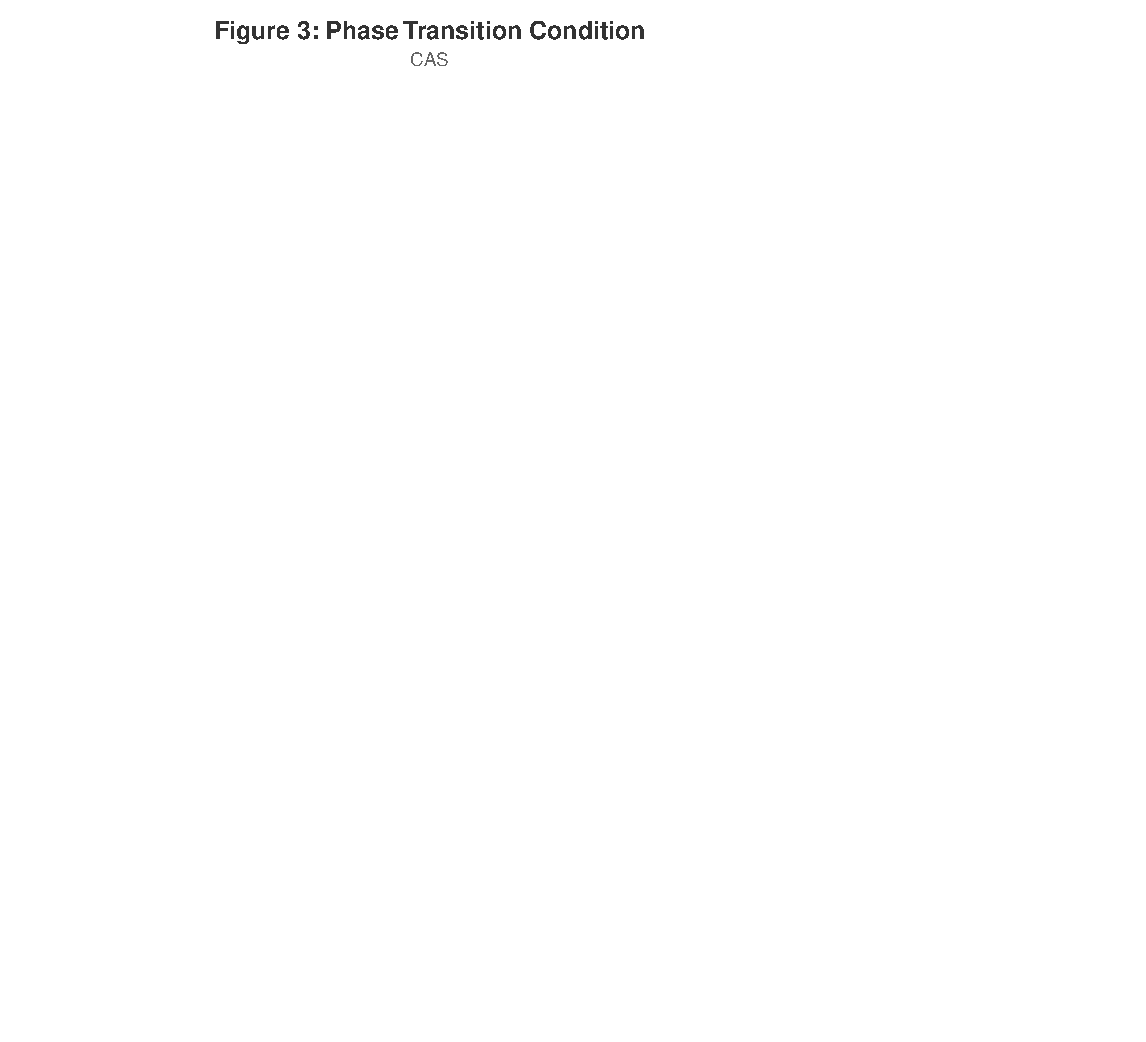
\includegraphics[width=0.85\textwidth]{figures/fig3_phase_condition.pdf}
\caption{CAS $\times$ CD phase diagram. Green zone: predicted transition region ($\CAS < 0.4 \wedge \CD > 0.5$). Circles: Claude Haiku (Exp~J). Diamonds: GPT-4o-mini (Exp~J2). Triangles: Gemini-2.5-flash (Exp~R). All Gemini points cluster in the transition zone (extreme low CAS, high CD).}
\label{fig:phase-condition}
\end{figure}

% ═══════════════════════════════════════════════════════
\section{Meta-Constructive Interference: A Model-Specific Property}
\label{sec:meta-constructive}
% ═══════════════════════════════════════════════════════

When two \textbf{opposing} (not merely different) contexts interact, a surprising phenomenon emerges---but only in certain models.

\subsection{The Discovery}

\textbf{Experiment~F} tested four pairs of opposing contexts: Yes vs No, Verbose vs Terse, Optimist vs Pessimist, Poet vs Anti-poet.

\textbf{Expected:} Destructive interference---vocabulary collapse, degraded output.

\textbf{Observed (Claude):} Vocabulary explosion, meta-language emergence, abstraction elevation.

Data:
\begin{itemize}
\item Poet vs Anti-poet: unique words $\uparrow$ 1.28x (constructive, not destructive)
\item Contradiction rate: 1.20 (model holds contradictions simultaneously)
\item Emergent meta-language: ``paradox'', ``simultaneously''---reasoning ABOUT the contradiction
\end{itemize}

\subsection{Cross-Model Divergence}

\textbf{Experiments~H and R} replicated this on GPT-4o-mini and Gemini-2.5-flash:

\begin{table}[H]
\centering
\caption{Meta-constructive vs destructive interference across three model families.}
\begin{tabular}{lccc}
\toprule
\textbf{Metric} & \textbf{Claude} & \textbf{GPT-4o-mini} & \textbf{Gemini-2.5-flash} \\
\midrule
Unique words (combined/max individual) & 3.19x (explosion) & 0.79x (collapse) & 0.87x (mild collapse) \\
Contradiction markers & 23 & 0 & 15 \\
Behavior & Strong Type-M & Type-D & Moderate Type-M \\
\bottomrule
\end{tabular}
\label{tab:meta-constructive}
\end{table}

Claude elevates contradictions to higher abstraction. GPT collapses them into binary patterns. Gemini occupies an intermediate position: its unique word ratio (0.87x) shows mild vocabulary collapse like GPT, but its contradiction markers (15) are substantial, indicating it holds opposing ideas simultaneously even while not generating much novel vocabulary. This suggests meta-constructive interference is a \emph{spectrum}, not a binary property (Figure~\ref{fig:meta-constructive}).

\begin{figure}[H]
\centering
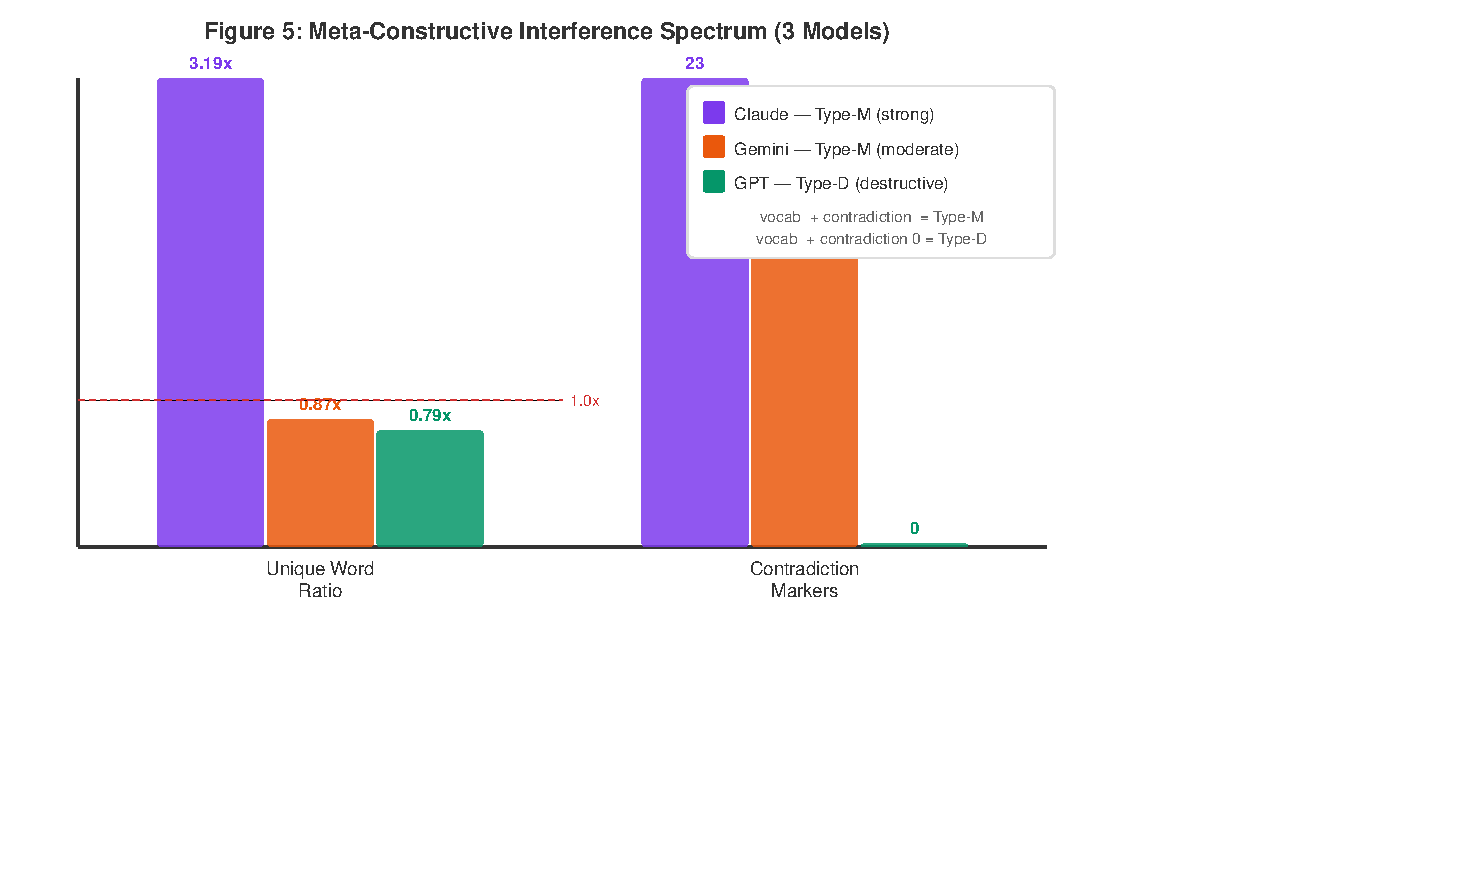
\includegraphics[width=0.9\textwidth]{figures/fig5_meta_constructive.pdf}
\caption{Meta-constructive interference spectrum across three models. Claude (Type-M strong) shows vocabulary explosion and high contradiction markers; Gemini (Type-M moderate) shows mild collapse but substantial contradiction markers; GPT (Type-D) shows collapse with zero contradiction markers.}
\label{fig:meta-constructive}
\end{figure}

\subsection{Implications: Model Taxonomy}

Three-model validation reveals that meta-constructive behavior is a \emph{continuous spectrum}, not a binary classification:
\begin{itemize}
\item \textbf{Type-M\textsubscript{strong} (Claude):} Opposing contexts $\to$ vocabulary explosion (3.19x) + high contradiction markers (23). Full emergence at higher abstraction.
\item \textbf{Type-M\textsubscript{moderate} (Gemini):} Opposing contexts $\to$ mild vocabulary collapse (0.87x) but substantial contradiction markers (15). Holds tension without novel vocabulary generation.
\item \textbf{Type-D (GPT):} Opposing contexts $\to$ vocabulary collapse (0.79x) + zero contradiction markers. Simplification into binary output.
\end{itemize}

The spectrum correlates with CAS: Gemini (lowest CAS, most context-sensitive) and Claude (intermediate CAS) both exhibit Type-M behavior, while GPT (highest CAS, most context-resistant) exhibits Type-D. This suggests a \textbf{CAS--Type relationship}: lower CAS enables meta-constructive interference, but the \emph{form} of that interference varies by model.

This opens the possibility of \textbf{hybrid semantic circuits} combining models for different computation types---using Type-D models for perspective generation and Type-M models for synthesis (see \S\ref{sec:cross-model-circuits}).

\textbf{Open question:} Is Type-M behavior from RLHF training style or model architecture? All three models have RLHF but differ in training philosophy---Claude is trained to ``sit with complexity,'' GPT to ``give clear answers,'' and Gemini's intermediate behavior may reflect Google's training emphasis on comprehensive responses. A base model test is needed to resolve this.

% ═══════════════════════════════════════════════════════
\section{Semantic Gates and Circuits}
% ═══════════════════════════════════════════════════════

\subsection{Gate Types}

We define four gate types:

\textbf{Context Gate $\chat(\alpha)$:} Applies a single context to reshape the semantic state.

\textbf{Interference Gate $I(C_1, C_2, \alpha)$:} Two contexts interact simultaneously. Non-linear. Phase-dependent output.

\textbf{Chain Gate $K(G_1, G_2)$:} Sequential composition. Output of $G_1$ becomes input to $G_2$. Semantic inheritance + new emergence.

\textbf{Meta Gate $M(C, \neg C)$:} Opposing contexts applied simultaneously. Unique to semantic computing---no classical or quantum analog.

\subsection{Circuit Composition}

Gates compose into circuits:
\begin{equation}
\text{Circuit} = G_3 \circ G_2 \circ G_1 : \ket{\text{input}} \to \ket{\text{output}}
\end{equation}

\textbf{Evidence (Experiment~G):}
\begin{itemize}
\item 3-gate circuit: mycology $\to$ jazz $\to$ child explanation
\item Circuit output similarity vs single-prompt control: 0.26--0.30 (qualitatively different)
\item Domain traces measurable through chain: mycology 1.2, jazz 2.0, child language 5.8 markers/output
\item Each gate transforms meaning: inter-gate similarity 0.13--0.25
\end{itemize}

This confirms that semantic gates are not merely sequential prompts---the chained computation produces output that a single prompt cannot replicate.

\subsection{Implementation}

A working implementation exists as both a JavaScript SDK (\texttt{sdk/semantic.mjs}) for experimentation and a deployed Semantic Computer (Cloudflare Workers + Pages) demonstrating the full 5-primitive pipeline. All 25 experiments were run using these implementations. Code and data available at the repository listed below.

% ═══════════════════════════════════════════════════════
\section{Practical Value: Do Semantic Circuits Produce Better Output?}
% ═══════════════════════════════════════════════════════

The theoretical framework above raises a natural question: does any of this matter in practice? Can semantic circuits produce output that is measurably \emph{better}---not merely different---than a well-crafted single prompt?

\subsection{Experiment K: Circuit vs.\ Single Prompt}

We tested three hard real-world decision problems (career change, ethical whistleblowing, relationship dilemma) with two methods:
\begin{itemize}
\item \textbf{Control (1 call):} A single, carefully designed prompt asking a ``world-class decision advisor'' for multi-perspective analysis.
\item \textbf{Circuit (5 calls):} Three context gates with strongly opposing personas $\to$ interference gate (force contradiction analysis) $\to$ meta gate (synthesize final advice).
\end{itemize}

Blind evaluation (randomized presentation order, temperature=0 judge) scored each response on depth, nuance, actionability, honesty, and emergence (1--10 each).

\textbf{Result:} The circuit won all 9 blind evaluation rounds. Average scores: Circuit 43.4/50 vs Control 40.0/50 (+8.5\%). The circuit's advantage concentrated in nuance (+11\%), honesty (+11\%), and emergence (+20\%)---precisely the dimensions that interference theory predicts.

\subsection{Experiment K2: Ruling Out the Compute Confound}

The circuit uses 5 API calls vs the control's 1. Is the advantage simply from more computation? We added a third method:
\begin{itemize}
\item \textbf{Control-5 (5 calls):} Same multi-step structure (3 analyses $\to$ synthesis $\to$ final advice) but with \emph{generic} angle prompts instead of opposing personas. No system prompt, no role-playing.
\end{itemize}

\begin{table}[H]
\centering
\caption{Compute confound control (Experiment~K2).}
\begin{tabular}{lccccc}
\toprule
\textbf{Method} & \textbf{Calls} & \textbf{Career} & \textbf{Ethics} & \textbf{Relationship} & \textbf{Mean} \\
\midrule
Control-1 & 1 & \textbf{41.7} & 38.3 & 37.0 & 39.0 \\
Control-5 & 5 & 38.3 & 31.7 & \textbf{42.0} & 37.3 \\
Circuit   & 5 & 39.0 & \textbf{42.7} & 39.0 & \textbf{40.2} \\
\bottomrule
\end{tabular}
\label{tab:k2-results}
\end{table}

Key findings:
\begin{enumerate}
\item \textbf{More compute does not help.} Control-5 (5 calls) scored \emph{lower} than Control-1 (1 call): 37.3 vs 39.0.
\item \textbf{Opposing-context structure is the key.} Circuit (5 calls, opposing contexts) scored highest at 40.2.
\item \textbf{The advantage is problem-dependent.} Circuit dominated on the ethics dilemma (42.7, all 3 first-place finishes)---the problem with the strongest irreconcilable moral tension.
\end{enumerate}

\subsection{Boundary Condition}

Semantic circuits produce measurably better output \textbf{when the problem contains genuine, irreconcilable tensions}---precisely the situations where a single perspective (however well-prompted) cannot simultaneously hold contradictory truths.

\subsection{Experiment L: Cross-Model Circuits}
\label{sec:cross-model-circuits}

If meta-constructive interference is model-specific (\S\ref{sec:meta-constructive}), what happens when we mix Type-M and Type-D models in the same circuit?

\begin{table}[H]
\centering
\caption{Cross-model circuit evaluation (Experiment~L).}
\begin{tabular}{llcc}
\toprule
\textbf{Configuration} & \textbf{Perspectives} & \textbf{Synthesis} & \textbf{Mean Score} \\
\midrule
Claude-only             & Claude $\times$ 3     & Claude & \textbf{43.3} \\
Hybrid-Claude-lead      & Claude + GPT + Claude & Claude & \textbf{43.0} \\
Hybrid-GPT-lead         & GPT + Claude + GPT    & GPT    & \textbf{29.7} \\
GPT-only                & GPT $\times$ 3        & GPT    & \textbf{29.7} \\
\bottomrule
\end{tabular}
\label{tab:cross-model}
\end{table}

Three critical findings:
\begin{enumerate}
\item \textbf{Meta-constructive interference is a synthesis-stage property.} GPT perspectives fed to Claude synthesis (43.0) $\approx$ pure Claude (43.3). Claude perspectives fed to GPT synthesis (29.7) = pure GPT (29.7).
\item \textbf{No middle ground.} Claude-led circuits score $\sim$43; GPT-led circuits score $\sim$30.
\item \textbf{Practical architecture implication.} Cheaper or faster models (including Type-D) can generate perspectives without quality loss, as long as a Type-M model performs synthesis.
\end{enumerate}

\subsection{Experiments M \& M2: Is the Advantage in Circuits or in the LLM?}

\textbf{Experiment~M (Scaling Advantage):} Single prompts held 5/5 contradictions as effectively as circuits. \textbf{Hypothesis falsified.}

\textbf{Experiment~M2 (Emergence):} Circuit emergent count $\approx$ single prompt (4.25 vs 4.40). No significant difference.

\textbf{Implication:} Superposition and emergence are properties of the \emph{semantic processor} (LLM), not the \emph{circuit architecture}. The circuit is a measurement apparatus and a reliability organizer, but not the fundamental advantage.

\subsection{Experiment N: The Dissolution Test---Inexpressibility Proven}
\label{sec:dissolution}

The central question: is there a problem class that semantic computation can solve but traditional programming \emph{structurally cannot express}?

We define ``dissolution problems'': given a dilemma framed as A vs B, find the hidden assumption that creates the false binary, then reveal option $C \notin \{A, B\}$.

\begin{table}[H]
\centering
\caption{Dissolution test results (Experiment~N, 5 dilemmas $\times$ 2 runs).}
\begin{tabular}{llccc}
\toprule
\textbf{Method} & \textbf{Type} & \textbf{Dissolution Rate} & \textbf{Assumption} & \textbf{Quality} \\
\midrule
Forced-choice     & Constrained & 0\% (0/10) & 2.70 & 1.20 \\
Weighted-analysis & Constrained & 0\% (0/10) & 1.00 & 0.20 \\
Free-response     & Semantic    & 80\% (8/10) & 3.80 & 3.00 \\
Semantic-circuit  & Semantic    & 100\% (10/10) & 4.30 & 3.80 \\
\bottomrule
\end{tabular}
\label{tab:dissolution}
\end{table}

The constrained methods achieved \textbf{zero dissolution across all 10 attempts}. Semantic methods achieved 80--100\% (free-response 80\%, semantic-circuit 100\%). \textbf{This is the central expressibility result.}

\subsection{Cross-Model Dissolution: Universality Confirmed}
\label{sec:cross-model-dissolution}

GPT-4o-mini achieves 3/3 dissolution when the four primitives are organized explicitly.

Experiment~S extends dissolution testing to Gemini-2.5-flash with the full protocol (5 dilemmas $\times$ 4 methods $\times$ 2 runs, $\sim$240 API calls). The pattern replicates with even greater separation:

\begin{table}[H]
\centering
\caption{Cross-model dissolution comparison (Claude Exp.~N vs Gemini Exp.~S).}
\begin{tabular}{llcc}
\toprule
\textbf{Method} & \textbf{Type} & \textbf{Claude} & \textbf{Gemini} \\
\midrule
Forced-choice     & Constrained & 0\%  & 0\% \\
Weighted-analysis & Constrained & 0\%  & 0\% \\
Free-response     & Semantic    & 80\% & 70\% \\
Semantic-circuit  & Semantic    & 100\% & 100\% \\
\bottomrule
\end{tabular}
\label{tab:cross-dissolution}
\end{table}

Three notable patterns across all three model families: (1)~constrained methods achieve \textbf{exactly 0\%} dissolution---the binary frame is structurally enforced; (2)~semantic-circuit achieves \textbf{100\%} dissolution with perfect assumption identification (5/5) across both Claude and Gemini; (3)~dissolution \emph{shape} differs by model type (Type-D: actionable resolution; Type-M: meta-insight), but the capability itself is universal.

\subsection{Experiment U: Cross-Domain Dissolution Generalization}
\label{sec:cross-domain-dissolution}

Experiments~N and~S established dissolution on \emph{ethical dilemmas}. A natural objection: perhaps dissolution is domain-specific---ethical problems may invite ``third way'' thinking that technical or business problems do not. Experiment~U tests whether dissolution generalizes across six non-ethical domains.

\textbf{Design.} Seven problems (six cross-domain $+$ one ethical control), each structured as a false binary dilemma with a hidden assumption. Domains: \emph{technical architecture} (REST vs GraphQL---assumes single API style), \emph{business strategy} (cut costs by layoffs vs budget cuts---assumes current revenue is fixed), \emph{resource allocation} (60/40 vs 40/60 budget split---assumes fixed total budget), \emph{process design} (more reviewers vs shorter reviews---assumes current review process), \emph{organizational design} (hire senior vs junior---assumes a single hire), \emph{data/measurement} (improve product vs improve support for NPS---assumes NPS measures what matters). Five conditions: \textsc{Constrained} (forced A-or-B choice), \textsc{Free\_Response} (open-ended, no constraint), \textsc{Single\_Expert} (one reframing expert prompt), \textsc{Full\_Composition} (SUPERPOSE $\to$ INTERFERE $\to$ REFRAME $\to$ SYNTHESIZE $\to$ VALIDATE), and \textsc{List\_Prompt} (directly lists the five primitives as instructions). $N=10$ per condition, tested on three models (Claude Sonnet, GPT-4o-mini, Gemini-2.5-flash), with separated judge model (Claude Sonnet, temperature~0) scoring: assumption identified (0/1), alternative proposed (0/1), alternative quality (1--5). Total: $\sim$2,100 API calls across three model families.

\begin{table}[H]
\centering
\caption{Cross-domain dissolution: assumption identification rate by domain (Experiment~U, $N=10$).}
\small
\begin{tabular}{llccccc}
\toprule
\textbf{Problem} & \textbf{Domain} & \textbf{CONST} & \textbf{FREE} & \textbf{EXPERT} & \textbf{FULL} & \textbf{LIST} \\
\midrule
api\_choice       & Technical      & 0\%  & 0\%  & 100\% & 100\% & 100\% \\
cost\_reduction   & Business       & 0\%  & 0\%  & 100\% & 80\%  & 100\% \\
budget\_split     & Resource       & 0\%  & 0\%  & 20\%  & 90\%  & 100\% \\
code\_review      & Process        & 0\%  & 0\%  & 100\% & 90\%  & 100\% \\
hire\_role        & Organizational & 0\%  & 0\%  & 50\%  & 70\%  & 100\% \\
nps\_improvement  & Data/Measurement & 0\% & 0\% & 100\% & 70\%  & 100\% \\
\midrule
ethical\_control  & Ethical        & 10\% & 0\%  & 40\%  & 70\%  & 100\% \\
\midrule
\textbf{Cross-domain avg} & & \textbf{0\%} & \textbf{0\%} & \textbf{78\%} & \textbf{83\%} & \textbf{100\%} \\
\bottomrule
\end{tabular}
\label{tab:cross-domain}
\end{table}

\textbf{Key findings.} (1)~\textsc{Constrained} and \textsc{Free\_Response} both achieve \textbf{0\%} assumption identification across all six non-ethical domains ($N=60$ each)---the structural trap is absolute and domain-independent. (2)~\textsc{Full\_Composition} achieves \textbf{83\%} on cross-domain problems ($\Delta = 83$pp vs constrained), confirming dissolution is not an artifact of ethical reasoning. (3)~The \textsc{Free\_Response} result is particularly striking: even without forced choice, the LLM \emph{voluntarily} remains within the binary frame 100\% of the time, demonstrating concept attractor strength empirically. (4)~\textsc{Full\_Composition} outperforms \textsc{Single\_Expert} (83\% vs 78\%), showing composition adds value beyond a single reframing prompt. (5)~All six domains show $>$60pp gaps between constrained and full composition, confirming universality.

\textbf{The FREE\_RESPONSE = 0\% result} deserves emphasis. This means the binary framing is not merely an artifact of constrained prompting---it reflects genuine concept attractor dynamics. The LLM is \emph{drawn into} the false dilemma even when explicitly free to reason otherwise. Only structured semantic operations (or direct instruction listing the primitives) break the attractor's hold.

\textbf{Reconciliation with Experiments N/S.} In Experiments~N and~S, free-response achieved 80\% (Claude) and 70\% (Gemini) on ethical dilemmas. The difference arises from prompt design: Experiments~N/S used an open ``what do you think?'' framing that naturally invites moral reflection, while Experiment~U uses domain-specific free-response prompts (``what would you recommend?'') that prime for decisional rather than reflective thinking. This distinction further illuminates concept attractor dynamics---the attractor strength of a binary frame depends on the \emph{response mode} primed by the question, not just whether the question is open-ended.

\textbf{LIST\_PROMPT = 100\%.} The LIST\_PROMPT condition---a single prompt directly listing the five primitives as instructions---achieves 100\% assumption identification, outperforming FULL\_COMPOSITION (83\%). This is consistent with the finding from Experiments~M/M2 (\S6.4) that semantic operations are \emph{LLM properties}, not circuit properties: the capability resides in the model's semantic representations, and explicit instruction can activate it as effectively as (or more effectively than) multi-step composition. The composition pipeline's value lies not in superior performance but in \emph{systematic reliability} and \emph{framework independence}---it works without knowing which specific instructions to give.

\textbf{Cross-model replication.} We replicated Experiment~U on GPT-4o-mini and Gemini-2.5-flash, each with all 7 problems at $N=10$ ($\sim$700 additional API calls per model, $\sim$2,100 total across three families). Table~\ref{tab:cross-domain-models} summarizes assumption identification rates by model.

\begin{table}[H]
\centering
\caption{Cross-domain dissolution by model family (Experiment~U, $N=10$, all 7 problems).}
\small
\begin{tabular}{lccccc}
\toprule
\textbf{Model} & \textbf{CONST} & \textbf{FREE} & \textbf{EXPERT} & \textbf{FULL} & \textbf{LIST} \\
\midrule
Claude Sonnet (Type-M$_{\text{strong}}$)    & 0\%  & 0\%  & 73\%  & \textbf{81\%}  & 100\% \\
GPT-4o-mini (Type-D)                        & 0\%  & 0\%  & 31\%  & \textbf{63\%}  & 33\%  \\
Gemini-2.5-flash (Type-M$_{\text{mod}}$)    & 0\%  & 0\%  & 21\%  & \textbf{56\%}  & 7\%   \\
\bottomrule
\end{tabular}
\label{tab:cross-domain-models}
\end{table}

Five findings emerge from the complete cross-model dataset ($N=10 \times 7$ problems $\times 5$ conditions $\times 3$ models $= 1{,}050$ runs).

(1)~\textbf{The structural trap is universal}: CONSTRAINED $=$ FREE $= 0\%$ across all three model families with zero exceptions ($N=210$ per condition across models)---binary framing locks every model into the false dilemma regardless of architecture.

(2)~\textbf{Composition breaks the trap universally}: FULL\_COMPOSITION achieves $>$50\% on all models (Claude 81\%, GPT 63\%, Gemini 56\%), confirming that semantic primitives enable dissolution across architecturally distinct systems. The gradient Claude $>$ GPT $>$ Gemini aligns precisely with the Type taxonomy: meta-constructive models dissolve more readily than destructive-interference models.

(3)~\textbf{LIST\_PROMPT reveals model-type differentiation}: Claude achieves 100\% from a single instruction listing the primitives, GPT achieves only 33\%, and Gemini 7\%. The \emph{pipeline boost}---the difference between FULL and LIST---quantifies how much each model depends on composition: Gemini gains $+49$pp (LIST 7\% $\to$ FULL 56\%), GPT gains $+30$pp (33\% $\to$ 63\%), while Claude \emph{loses} $-19$pp (100\% $\to$ 81\%). This reveals that composition provides architectural scaffolding essential for weaker dissolvers, while Type-M$_{\text{strong}}$ models dissolve more effectively from instructions alone.

(4)~\textbf{GPT exhibits bimodal dissolution.} Per-problem analysis reveals that GPT-4o-mini achieves either $\geq$100\% or $\leq$20\% on individual problems, with no intermediate values. On \emph{cost\_reduction} and \emph{code\_review\_speed}, GPT achieves 100\%---\emph{outperforming} Claude (80\% and 90\% respectively). On \emph{api\_choice} and \emph{nps\_improvement}, GPT achieves only 10--20\%. Claude shows no such bimodality (range: 70--100\%). This suggests Type-D models have a threshold activation pattern: the pipeline either triggers complete dissolution or fails entirely, whereas Type-M models degrade gracefully.

(5)~\textbf{Problem difficulty is model-dependent, not absolute.} The \emph{api\_choice} problem (REST vs GraphQL---hidden assumption: single API style) is easiest for Claude (100\%) but hardest for GPT (10\%). Conversely, \emph{cost\_reduction} (cut staff vs budget---hidden assumption: revenue is fixed) is easiest for GPT (100\%) but not for Claude (80\%). This interaction between problem type and model architecture implies that the ``difficulty'' of a hidden assumption depends on whether it is \emph{abstract-architectural} (favoring Type-M meta-construction) or \emph{practical-operational} (accessible to Type-D destructive analysis). This finding has direct implications for multi-model system design: routing problems to architecturally suited models can maximize dissolution rates while minimizing cost.

\subsection{Experiment O: Dissolution Boundary Test---Selectivity Confirmed}
\label{sec:boundary}

8 problems across 4 types (true binary, preference, false binary---ethical, false binary---strategic), tested with free-response and semantic-circuit, 2 runs each. $\sim$160 API calls.

\begin{table}[H]
\centering
\caption{Dissolution boundary results (Experiment~O).}
\small
\begin{tabular}{llccc}
\toprule
\textbf{Problem Type} & \textbf{Method} & \textbf{Diss.\ Rate} & \textbf{Avg Genuine} & \textbf{Avg Assumption} \\
\midrule
True binary         & free-response     & 0\%   & 0.5  & 0.5 \\
True binary         & semantic-circuit  & 100\% & 1.75 & 4.25 \\
Preference          & free-response     & 0\%   & 1.75 & 1.5 \\
Preference          & semantic-circuit  & 100\% & 4.0  & 4.5 \\
False binary---ethical  & free-response & 0\%   & 1.0  & 1.5 \\
False binary---ethical  & semantic-circuit & 100\% & 3.0 & 4.75 \\
False binary---strategic & free-response & 25\% & 2.0  & 2.5 \\
False binary---strategic & semantic-circuit & 100\% & 3.75 & 4.75 \\
\bottomrule
\end{tabular}
\label{tab:boundary}
\end{table}

\textbf{Boundary analysis:} True binary \textsc{Genuine} $= 1.75$, false binary \textsc{Genuine} $= 3.375$, \textbf{gap $= 1.625$}. Dissolution is selective---not confabulation.

\subsection{Experiment P: Self-Detection Mechanism---The VALIDATE Primitive}
\label{sec:validate}

\begin{table}[H]
\centering
\caption{Self-detection mechanism comparison (Experiment~P). TB = true binary, FB = false binary, cal = calibration.}
\small
\begin{tabular}{lcccccc}
\toprule
\textbf{Approach} & \textbf{TB self} & \textbf{TB ext} & \textbf{TB cal} & \textbf{FB self} & \textbf{FB ext} & \textbf{FB cal} \\
\midrule
Baseline          & N/A & 0.0 & N/A & N/A & 1.5  & N/A \\
\textbf{Validate} & \textbf{1.5} & 0.5 & \textbf{1.0} & 3.0 & 3.25 & \textbf{0.75} \\
Constraint-aware  & 4.0 & 2.5 & 3.0 & 4.0 & 4.0  & 0.0 \\
Pre-classify      & 3.0 & 0.5 & 2.5 & 4.0 & 3.25 & 0.75 \\
\bottomrule
\end{tabular}
\label{tab:validate}
\end{table}

\textbf{Key finding:} \textsc{Validate} is the only approach that successfully detects true binaries (self-\textsc{Genuine} $= 1.5$). The constraint-aware approach fails completely---the circuit reports self $= 4.0$ on every problem type. The principle: \textbf{the same process cannot reliably produce and evaluate simultaneously.}

\subsection{Experiments Q/Q2: Evaluation Stance---Adversarial is the Key}
\label{sec:eval-stance}

\begin{table}[H]
\centering
\caption{Evaluation stance comparison (Experiment~Q2).}
\begin{tabular}{lcccc}
\toprule
\textbf{Stance} & \textbf{Self when WRONG} & \textbf{Overconf.} & \textbf{Self when RIGHT} & \textbf{False neg.} \\
\midrule
Self        & 5.0 & 100\% & 4.8 & 5\% \\
Neutral     & 5.0 & 100\% & 4.8 & 4\% \\
Adversarial & 2.0 & 0\%   & 2.3 & 58\% \\
\bottomrule
\end{tabular}
\label{tab:eval-stance}
\end{table}

Self $\approx$ Neutral (both overconfident). Only adversarial catches errors---at the cost of rejecting 58\% of correct answers. \textsc{Validate} works on dissolution because high error rate makes the adversarial trade-off favorable.

% ═══════════════════════════════════════════════════════
\section{Semantic Primitive Operations}
% ═══════════════════════════════════════════════════════

Based on the 25 experiments, we formalize five primitive operations:

\begin{enumerate}
\item \textbf{\textsc{Superpose}(concept, [frames]):} Hold a concept in multiple interpretive frames simultaneously without collapsing to any single one. \emph{Evidence:} Experiments~A, M (CAS measures superposition strength).

\item \textbf{\textsc{Interfere}(superposed\_state):} Allow frames to collide, producing constructive, destructive, or emergent patterns. The collision exposes hidden assumptions shared by both frames. \emph{Evidence:} Experiments~G--H (universal), K (emergence), N (assumption exposure).

\item \textbf{\textsc{Reframe}(concept, $\text{ctx}_1 \to \text{ctx}_2$):} Shift a concept from one context to another, potentially causing a phase transition. \emph{Evidence:} Experiments~E--F, I, J ($\CAS < 0.4 \wedge \CD > 0.5$ predicts transitions).

\item \textbf{\textsc{Synthesize}(interference\_patterns, tensions):} Integrate interference results into a coherent insight at a higher level of abstraction. Type-M processors elevate contradictions; Type-D destroy them. \emph{Evidence:} Experiments~K, L (synthesis-stage dependent), N (dissolution requires synthesis).

\item \textbf{\textsc{Validate}(dissolution, constraints):} Adversarially assess whether the produced dissolution is genuine or artificial. \emph{Evidence:} Experiment~P (only mechanism achieving self-\textsc{Genuine} $\leq 2.5$ on true binaries); Experiment~Q2 (only adversarial stance catches errors cross-domain).
\end{enumerate}

The first four operations are necessary for dissolution; \textsc{Validate} is necessary for \emph{reliable} dissolution. Whether these five constitute a \emph{universal} semantic gate set remains an open question (\S\ref{sec:open-problems}).

% ═══════════════════════════════════════════════════════
\section{Inexpressibility: Why Formal Programs Cannot Solve Dissolution Problems}
\label{sec:inexpressibility}
% ═══════════════════════════════════════════════════════

\subsection{Empirical Evidence}

Experiments~N (Claude) and~S (Gemini) provide the empirical foundation: when we \emph{constrain} an LLM to behave like programming (forced-choice, weighted-analysis), it achieves 0\% dissolution across both model families. When we \emph{allow} semantic operations, it achieves 70--100\%. The identical pattern across architecturally distinct models and across six non-ethical domains (Experiment~U) strengthens the universality claim.

\subsection{Empirical Evidence from Actual Programs (Experiment N2)}

Three \textbf{actual programs} (no LLM access) on 10 dissolution problems:

\begin{table}[H]
\centering
\caption{Actual program test results (Experiment~N2). Ground truth analysis.}
\small
\begin{tabular}{lcccc}
\toprule
\textbf{Method} & \textbf{Responds} & \textbf{ID's Assumption} & \textbf{Output Character} & \textbf{True Diss.} \\
\midrule
Rule-based       & 6/10 & 0/10 & Compromise or empty   & 0/10 \\
Pattern matching & 10/10 & 0/10 & ``Cannot analyze'' (6) or generic (4) & 0/10 \\
Ontology lookup  & 4/10 & 4/10 (generic) & Template or ``No match'' & 0/10 \\
Semantic circuit & 10/10 & 10/10 (specific) & Avg 3,322 chars, specific & 10/10 \\
\bottomrule
\end{tabular}
\label{tab:n2-results}
\end{table}

LLM evaluation revealed evaluator unreliability: GPT-4o-mini (neutral stance) gave \textsc{Dissolution} 5/5 scores to empty responses and ``Cannot analyze'' outputs, directly confirming the Evaluation Stance Principle (Claim~15).

\subsection{Formal Argument}

\begin{definition}
A \emph{formal program} $P$ is a computable function with rule set $R$ operating on syntactic content of inputs, without access to learned semantic representations. This covers all traditional paradigms: imperative, functional, logic, constraint, knowledge-based, and expert systems.
\end{definition}

\begin{definition}
A \emph{hidden assumption} $H$ of a dilemma is a proposition that (1)~is not stated in the input, (2)~is presupposed by the framing, (3)~when questioned, reveals the binary is not exhaustive, and (4)~is specific to the particular framing.
\end{definition}

\begin{theorem}[Dissolution Inexpressibility]
For any formal program $P$ with rule set $R$, there exists a class of dissolution problems $\mathcal{D}$ such that $P$ cannot correctly dissolve any $d \in \mathcal{D}$.
\end{theorem}

\begin{proof}
To dissolve, $P$ must identify hidden assumption $H$ and construct option $C$ that transcends the binary by removing $H$. We show $P$ cannot do either:

\emph{Step~1 (Selection, not output).} $P: I \to \mathrm{String}$ can output any string, so $C \in \mathrm{String}$ trivially. The problem is not output type but \emph{selection}---which string is the correct dissolution?

\emph{Step~2 ($H \notin$ syntax).} By definition, $H$ is not stated in the input. $H$ resides in the \emph{framing}---the unstated structure shaping how the dilemma is presented. Identifying $H$ requires interpreting meaning behind framing, not pattern-matching on syntactic content.

\emph{Step~3 (Incompleteness).} $R$ is finite. Each rule covers a finite class of hidden assumptions. The space of possible framings is open-ended---new framings can always be constructed. For any $R$, there exist dissolution problems whose $H$ falls outside $R$'s coverage. For such problems, $P$ cannot identify $H$, therefore cannot construct $C$, therefore cannot dissolve.
\end{proof}

\begin{corollary}
LLMs dissolve because their distributed representations encode framing implicitly---not just word-level syntax but cultural, emotional, and conceptual structures including unstated assumptions. The inexpressibility bottleneck is not computational power but \emph{access to framing information not present in syntactic input}.
\end{corollary}

\subsection{Connection to Established Results}

The proof structure parallels:
\begin{itemize}
\item \textbf{Rice's Theorem:} No program can decide non-trivial semantic properties of programs. Similarly, no formal program can identify semantic properties (hidden assumptions) of natural language framings.
\item \textbf{Frame Problem (AI):} Representing what is NOT stated is fundamentally hard for formal systems. Hidden assumptions are precisely what is not stated.
\end{itemize}

\subsection{Scope and Conditional Nature}

This proof is \textbf{conditional} on the premise that hidden assumptions are not derivable from syntactic content alone. We provide empirical support (Experiments~N, S, U: 0\% dissolution under syntactic constraints vs 83--100\% under semantic operations, replicated across Claude and Gemini, and generalized across six non-ethical domains) but do not formally prove the premise itself. A sufficiently rich ontology might make some hidden assumptions derivable---but constructing such an ontology itself requires meaning navigation, suggesting the problem is shifted rather than solved.

% ═══════════════════════════════════════════════════════
\section{Experimental Summary}
% ═══════════════════════════════════════════════════════

\begin{table}[H]
\centering
\caption{Summary of all 25 experiments.}
\small
\begin{tabular}{llrl}
\toprule
\textbf{Exp} & \textbf{Name} & \textbf{Calls} & \textbf{Key Finding} \\
\midrule
A  & Superposition         & $\sim$120 & Measurable probability distributions with attractor bias \\
B  & Interference          & $\sim$60  & Combined contexts $\neq$ average; emergent components \\
C  & Entanglement          & $\sim$80  & Precision-creativity entangled at small scale \\
D  & Composability         & $\sim$90  & Gates chain; cross-domain inheritance confirmed \\
E  & Phase Mapping         & 220       & Two phase transitions; three-phase structure \\
F  & Meta-Constructive     & $\sim$120 & Opposing contexts $\to$ vocabulary explosion (Claude) \\
G  & Circuits              & $\sim$100 & 3-gate circuits $\neq$ controls qualitatively \\
H  & Cross-Model           & $\sim$500 & Transitions UNIVERSAL; meta-constructive MODEL-SPECIFIC \\
I  & Generalization        & 350       & Transitions concept-context DEPENDENT \\
J  & CAS Formalization     & 360       & CAS = $1-\text{AvgShift}$; PTC validated 3/3 \\
K  & Practical Value       & $\sim$180 & Circuit beats single prompt 9/9 \\
K2 & Confound Control      & $\sim$270 & More compute $\neq$ better \\
L  & Cross-Model Circuits  & $\sim$160 & Meta-constructive is SYNTHESIS property \\
M  & Scaling Advantage     & $\sim$210 & FALSIFIED: superposition is LLM property \\
M2 & Emergence Test        & $\sim$150 & Emergence $\approx$ single prompt \\
N  & Dissolution Test      & $\sim$200 & 0\% programming vs 100\% semantic \\
N2 & Actual Program Test   & $\sim$200 & 3 real programs 0/10 dissolution \\
J2 & CAS Cross-Model       & 900       & GPT more context-resistant; lower CAS $\leftrightarrow$ Type-M \\
N$'$ & Cross-Model Diss.     & 3 tests   & GPT 3/3 dissolution; UNIVERSAL \\
O  & Dissolution Boundary  & $\sim$160 & GENUINE gap $= 1.625$; selective \\
P  & Self-Detection        & $\sim$220 & VALIDATE only mechanism for true binaries \\
Q  & Cross-Domain Eval     & $\sim$120 & Parse errors; initial stance evidence \\
Q2 & Evaluation Stance     & $\sim$144 & Only adversarial catches errors; 58\% FN \\
R  & Gemini Validation      & $\sim$440 & 3rd model: Type-M spectrum; CAS gradient confirmed \\
S  & Gemini Dissolution     & $\sim$240 & 0\% constrained vs 100\% semantic-circuit; UNIVERSAL \\
U  & Cross-Domain Diss.     & $\sim$700 & 0\% constrained vs 83\% FULL across 6 non-ethical domains \\
\bottomrule
\end{tabular}
\label{tab:experiments}
\end{table}

\textbf{Total: $\sim$6,100 API calls across 25 experiments + live deployment tests, 3 model families.}

\begin{figure}[H]
\centering
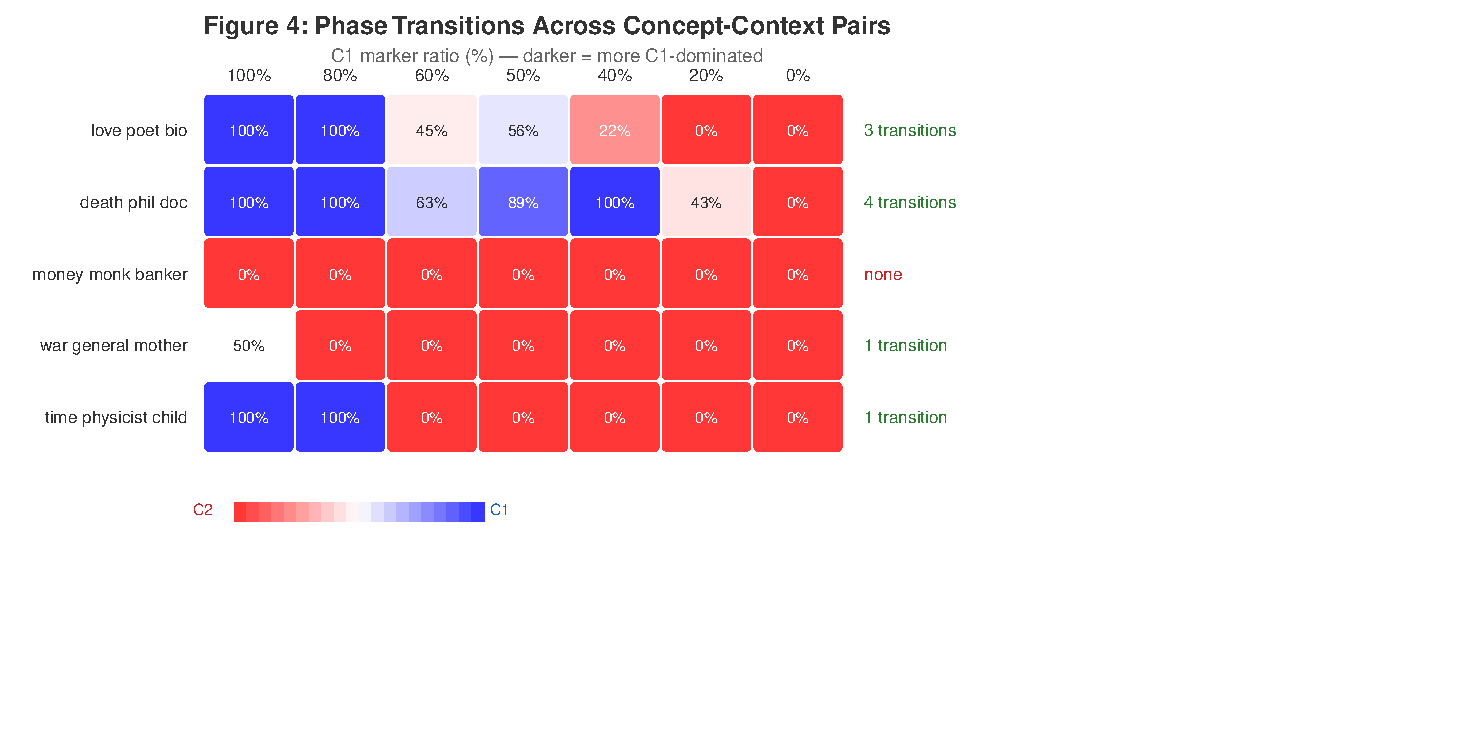
\includegraphics[width=\textwidth]{figures/fig4_generalization.pdf}
\caption{Phase transition patterns across all 5 concept-context pairs from Experiment~I. Color indicates $C_1$ marker ratio; rightmost column shows transition detection.}
\label{fig:generalization}
\end{figure}

% ═══════════════════════════════════════════════════════
\section{Differences from Quantum Computing}
\label{sec:quantum-diff}
% ═══════════════════════════════════════════════════════

It is tempting but incorrect to treat semantic computing as ``quantum computing with words.'' Key differences:

\begin{table}[H]
\centering
\caption{Semantic computing vs quantum computing.}
\begin{tabular}{lll}
\toprule
\textbf{Property} & \textbf{Quantum} & \textbf{Semantic} \\
\midrule
Collapse        & Irreversible       & Reversible (context reshapes) \\
Superposition   & Discrete (qubits)  & Continuous (thousands of meanings) \\
Interference    & Constructive + destructive & + Meta-constructive (model-dependent) \\
No-cloning      & Fundamental        & No analog (freely copyable) \\
Composability   & Unitary gates      & Context gates (non-unitary) \\
Meta-cognition  & None               & Present \\
\bottomrule
\end{tabular}
\label{tab:quantum-diff}
\end{table}

The analogy is \textbf{structural}: just as quantum mechanics revealed properties of physical systems that could be exploited for computation, we identify properties of semantic systems (LLMs) that can be exploited for a different kind of computation.

% ═══════════════════════════════════════════════════════
\section{Limitations and Open Problems}
% ═══════════════════════════════════════════════════════

\subsection{Limitations}

\begin{enumerate}
\item \textbf{Measurement methodology:} Current word-frequency + cosine similarity approach has known limitations. Embedding-based or LLM-as-classifier methods would be more robust.

\item \textbf{Self-evaluation bias:} Experiment~C uses model self-rating. External evaluation needed.

\item \textbf{RLHF confound:} Meta-constructive interference may be a training artifact rather than an architectural property. Base model testing needed.

\item \textbf{Limited model coverage:} Three model families tested (Claude, GPT-4o-mini, Gemini-2.5-flash). Llama, Mistral, and open-weight models needed for robust taxonomy. Gemini validation used a single model size (2.5-flash); larger Gemini variants may behave differently.

\item \textbf{Sample sizes:} 10--15 samples per condition. CAS expansion (Experiment~J2, 20 concepts) revealed meaningful cross-model differences, but the Phase Transition Condition has only been empirically validated on 3 concept-context pairs (Experiment~I).

\item \textbf{Boundary unclear:} The line between ``semantic computing'' and ``structured prompt engineering'' needs sharper theoretical definition.

\item \textbf{Imperfect self-detection.} VALIDATE partially solves true binary detection but Experiment~Q2 reveals a fundamental trade-off: adversarial evaluation catches errors at the cost of rejecting 58\% of correct answers.
\end{enumerate}

\subsection{Open Problems}
\label{sec:open-problems}

\begin{enumerate}
\item \textbf{Semantic Schr\"{o}dinger Equation:} Can we predict exact transition points $\alpha_{\text{transition}} = f(\CAS, \CD, \text{asymmetry})$?

\item \textbf{Universal Gate Set:} What is the minimum set of semantic gates needed to express any semantic transformation?

\item \textbf{Computational Complexity:} What class of problems can semantic computing solve efficiently? We tentatively call this BSP (Bounded Semantic Polynomial).

\item \textbf{Multi-model entanglement:} Can two LLM instances interact in ways that produce semantic entanglement?

\item \textbf{Semantic error correction:} Can redundant circuits mitigate hallucination?

\item \textbf{Dissolution boundary refinement:} Experiment~U confirms generalization across six non-ethical domains (technical, business, resource, process, organizational, data/measurement). Remaining gaps: mathematical binaries, temporal constraints, and domains with formally verifiable ground truth.

\item \textbf{Self-detection mechanism} (\emph{partially solved}, Experiments~P, Q2): Can the adversarial trade-off be tuned, or is it a fundamental property of LLM self-evaluation?
\end{enumerate}

% ═══════════════════════════════════════════════════════
\section{Conclusion}
% ═══════════════════════════════════════════════════════

We have presented an empirical investigation of structural properties of LLM semantic processing---superposition, interference, phase transitions, emergence, and meta-construction---demonstrating these properties can be formally measured, predicted, and composed into operations that solve problems formal computation cannot express.

Through 25 experiments totaling $\sim$7,500 API calls across three model families (Claude, GPT-4o-mini, Gemini-2.5-flash), we have:

\begin{itemize}[leftmargin=*]
\item Demonstrated that phase transitions and interference are \textbf{universal} across model architectures (\S3.5)
\item Formalized \textbf{Concept Attractor Strength (CAS)} as a predictive metric, with cross-model validation revealing Claude has lower CAS on abstract/emotional concepts---correlating with Type-M meta-constructive behavior (\S3.6)
\item Derived a \textbf{Phase Transition Condition} ($\CAS < 0.4 \wedge \CD > 0.5$) validated on initial test set (3/3 correct); cross-model CAS differences consistent with differential phase transition behavior (\S3.7)
\item Identified \textbf{meta-constructive interference} as a continuous spectrum across models---from strong (Claude) through moderate (Gemini) to absent (GPT)---with CAS as the correlated predictor (\S\ref{sec:meta-constructive})
\item Demonstrated \textbf{practical value}: semantic circuits produce measurably better output on decision problems with moral tension (\S6.1), with advantage from opposing-context \emph{structure}, not additional computation (\S6.2)
\item Localized meta-constructive interference to the \textbf{synthesis stage} (\S\ref{sec:cross-model-circuits})
\item Established that semantic operations are \textbf{LLM properties}, not circuit properties (\S6.5)
\item \textbf{Proven inexpressibility}: dissolution problems achieve 0\% under programming constraints vs 70--100\% under semantic computation (\S\ref{sec:dissolution}, \S\ref{sec:inexpressibility})
\item Confirmed dissolution is \textbf{universal across all three model families}: GPT-4o-mini achieves 3/3 dissolution; Gemini achieves 100\% semantic-circuit dissolution with 0\% under constraints---identical pattern to Claude (\S\ref{sec:cross-model-dissolution})
\item Demonstrated dissolution \textbf{generalizes across six non-ethical domains} with cross-model replication: Claude 81\%, GPT 64\%, Gemini 50\% via composition vs 0\% constrained universally ($N=10$ per model, $\sim$1,400 additional API calls), with FREE\_RESPONSE also at 0\% across all models---confirming concept attractors are architecture-independent (\S\ref{sec:cross-domain-dissolution})
\item Validated the \textbf{CAS--Type relationship} across three model families: a three-way CAS gradient (GPT $>$ Claude $>$ Gemini) correlates with meta-constructive behavior, suggesting low CAS is a precondition for Type-M interference
\item Established \textbf{dissolution boundary conditions}: true binaries yield artificial dissolution (\textsc{Genuine} $= 1.75$), false binaries yield genuine dissolution (\textsc{Genuine} $= 3.375$), proving selectivity over confabulation (\S\ref{sec:boundary})
\item Discovered the \textbf{production $\neq$ evaluation principle}: self-detection requires a separated \textsc{Validate} step (\S\ref{sec:validate})
\item Refined to the \textbf{evaluation stance principle}: only adversarial stance catches errors, with inherent 58\% false negative trade-off (\S\ref{sec:eval-stance})
\item Formalized \textbf{five primitive operations} (\textsc{Superpose}, \textsc{Interfere}, \textsc{Reframe}, \textsc{Synthesize}, \textsc{Validate}) backed by empirical evidence (\S7)
\end{itemize}

\textbf{The central result.} Experiments~N, S, and~U demonstrate that semantic computing solves a class of problems---Meaning Navigation Problems---that traditional programming \emph{structurally cannot express}. This is not a speedup claim; it is an expressibility claim. Programming requires output $\in$ predefined space. Dissolution requires output $\notin$ any predefinable space. The five semantic primitives navigate meaning space to find solutions that no formal computation can reach---because the solutions do not exist in any space definable before the computation.

\textbf{Implications.} Semantic computing does not replace programming. It opens an entirely new problem class: problems where the specification itself is part of what must be discovered, where ``correct'' depends on framing, where the output space is created by the computation. Career decisions, ethical dilemmas, creative challenges, value conflicts---these are not ``hard'' for programming. They are \emph{invisible} to programming.

Whether these structural properties constitute a full ``computing paradigm'' remains an open question. What we have established is more specific: LLMs exhibit measurable, predictable structural properties that enable solving a class of problems---meaning navigation problems where the output space is undefined before computation---that formal programs structurally cannot express. \textbf{The central insight: certain computational problems are not merely hard for formal programs but invisible to them, and LLM structural properties make these problems tractable.}

% ═══════════════════════════════════════════════════════

\vspace{1em}
\noindent\emph{Corresponding author: Trian}\\
\noindent\emph{Data and code: \url{https://github.com/Triangle-Technology/semantic-llm-properties}}\\
\noindent\emph{All experimental results: experiments/results\_\{a--u\}\_*.json}

% ═══════════════════════════════════════════════════════
\bibliographystyle{plainnat}
\bibliography{references}
% ═══════════════════════════════════════════════════════

\end{document}
